%!TEX root = main_acm.tex

\section{Analyzing Misclassification}
\label{sec:inaccu}

After using BGP-related features to classify anycast and unicast prefixes, we
further inspect the instances of false negative (anycast prefixes wrongly
labeled as unicast prefixes) and false positive (unicast prefixes wrongly
labeled as anycast prefixes) to understand the causes of inaccuracy. For false
negatives (0.05\% and 0.03\% in the decision tree and random forest classifiers
respectively), we identify that they are mainly caused by geographically distributed
autonomous systems.  By manually examining false positives
(10.55\% and 10.48\%), we find that the
anycast dataset we used does miss some cases that are highly likely to be
anycast. Also, we discover that the emerging remote peering introduces
unintended impact on the anycast routing, which essentially reduces the
distinction between anycast and unicast in our BGP-related features.

The distributions of the studied features of false positives (FP) and false
negatives (FN) are also presented in Figure~\ref{fig_FP_FN}, which  shows that
the feature distributions of FN are similar to those of anycast prefixes and the
feature distributions of FP are similar to those of unicast prefixes.

\begin{table}[t]
\begin{minipage}{.5\linewidth}
\centering
\caption{Anomaly in FN}
\small
\label{tab_FN}
\begin{tabular}{ | c | c | c | }
\hline
Feature & Value & \% in FN \\
\hline
\textbf{\texttt{N}} & 1 & 46.80\\ 
\hline
\textbf{\texttt{P1}}$|_{N\neq1} $ & 0 & 18.90 \\
\hline
\textbf{\texttt{P2}}$|_{N\neq1,P1\neq0} $ & 0 & 14.82 \\
\hline
\textbf{\texttt{MD}} & $\leq$ 4 & 82.27 \\
\hline
\textbf{\texttt{ML}} & $>$ 3 & 57.85\\
\hline
\end{tabular}
\vspace{-3pt}
\end{minipage}\hfill
\begin{minipage}{.5\linewidth}
    \centering
    \caption{Anomaly in FP}
    \small
    \label{tab_FP}
\begin{tabular}{ | c | c | c | }
\hline
Feature & Value & \% in FP \\
\hline
\textbf{\texttt{N}} & $>$ 3 & 99.06\\ 
\hline
\textbf{\texttt{P1}} & $\geq$ 0.5 & 82.22 \\
\hline
\textbf{\texttt{P2}} & $\geq$ 0.07 & 77.78 \\
\hline
\textbf{\texttt{MD}} & $\geq$ 4 & 78.09 \\
\hline
\textbf{\texttt{ML}} & $\leq$ 3 & 77.78\\
\hline
\end{tabular} 
\vspace{-3pt}
\end{minipage}
\end{table}

\vspace{2pt}
\textbf{False Negative (FN)}. We misclassify 344 anycast prefixes as unicast.
Table~\ref{tab_FN} shows that several FN features have values that are very
different from those we find in near-ground-truth data (shown in
Figure~\ref{fig_FP_FN}).
For example, based on our heuristics, anycast prefixes should have relatively
large N and P1, i.e., more upstream ASes and more pairs with long distance.
However, in FN we observe 46.80\% of prefixes with only one upstream AS (N=1).
We use RIPEstat Geoloc tool~\cite{RIPE_GEO} and MaxMind's GeoLite City
Dataset~\cite{MaxMind} to examine the geo-locations of these upstream ASes, and find that all 24 ASes appear in at least three different locations, indicating that an upstream AS whose geographic presence is largely distributed would cause such misclassifications.

Furthermore, given N $\neq$ 1, there are still 18.90\% of anycast prefixes in FN with P1=0 (i.e., no upstream AS pair with the distance greater than 1).
This could be because some anycast prefixes are not globally distributed (i.e., \textit{regional} anycast deployment~\cite{hao2018}), resulting in upstream ASes that are close. Such concentration can contribute to abnormal values for P2, MD, and ML as well.


\vspace{2pt}
\textbf{False Positive (FP)}. For false positives, the abnormal feature values and percentage of the prefixes with such values are shown in Table~\ref{tab_FP}. Table~\ref{tab_FP} shows that the feature values of such ``unicast'' prefixes are similar to those of anycast prefixes.
One possible reason is that these false positives are indeed anycast prefixes
but have been wrongly labeled as unicast in the near-ground-truth dataset, which has been actually obtained using a conservative classification approach, avoiding labeling prefixes as anycast when active measurements provide insufficient evidence~\cite{cicalese2015characterizing}.

We investigate which organizations originate these prefixes. Figure~\ref{FP_owners} shows the owners that possess at least 2 FP prefixes. We observe that 87.3\% of false positive prefixes belong to IT companies or infrastructure providers. It is very likely that such organizations have deployed anycast-based services. To validate this intuition, we traceroute to these prefixes from distributed vantage points from RIPE Atlas (in US, Brazil, Japan, Australia, South Africa, and Netherlands). We successfully reach 117 out of 318 FP prefixes. We then leverage the IP geolocation and latency measurements to manually infer the types of these prefixes based on speed-of-light violations. Among these 117 prefixes, 31 of them show strong evidence of anycast routing. Therefore, some of the false positives we obtained are actually true positives, due to the incompleteness of the anycast near-ground-truth dataset (which indeed has been generated using a conservative approach \cite{cicalese2015characterizing}).

However, we do find that several unicast prefixes show a very similar deployment pattern to anycast. By mining the corresponding AS paths and the IP geolocation of intermediate network nodes from traceroutes, we speculate that the main cause is the emerging remote peering deployment. We find that 28.61\% (91 out of 318) of the false positives might be caused by remote peering (\S\ref{sub:idRP}). For these 91 unicast prefixes, the average values of {\sf N}, {\sf P1},  {\sf P2}, {\sf MD}, and {\sf ML} are 7, 0.38, 0, 2, and 6, respectively. These numbers indicate that remote peering will blur the distinction of our features between unicast and anycast. We present a detailed study of the potential impact of remote peering on anycast routing in \S\ref{sec:rp}.

\begin{figure}[h]
\vspace{-6pt}
	\centerline{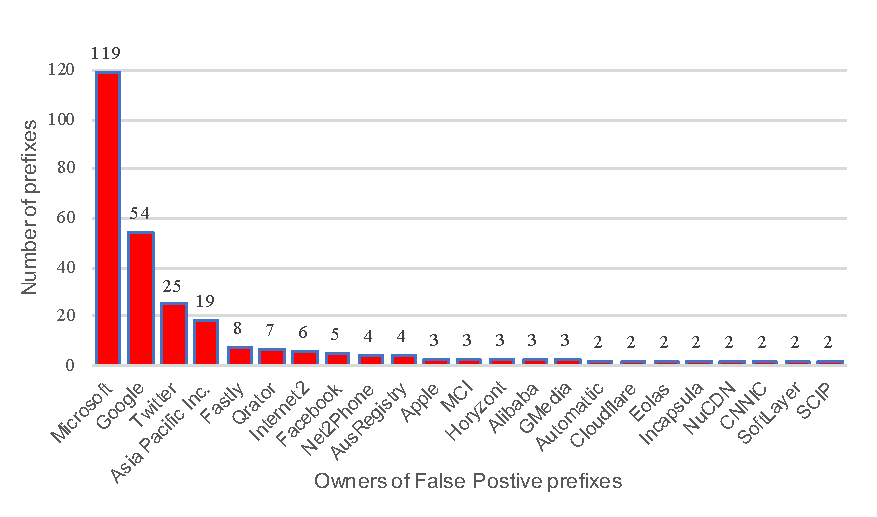
\includegraphics[scale=0.58]{fig/FP_owners.pdf}}
	\caption{Breakdown of the Owners of False Positive Prefixes}
	\label{FP_owners}
\end{figure}
